 \documentclass[landscape, 8pt]{extarticle}
\usepackage{geometry}
% \usepackage{showframe}

\geometry{
    a4paper, 
    margin=0.17in
}

\usepackage{graphicx} % Required for inserting images
\usepackage{amsmath}
\usepackage{amsfonts}
\usepackage{amssymb}
\usepackage{preamble}
\usepackage{multicol}
\usepackage{lipsum}
\usepackage[framemethod=TikZ]{mdframed}
\usepackage{thmboxes}
\usepackage{float}
% \usepackage{setspace}
\usepackage[nodisplayskipstretch]{setspace}

% \setlength{\parskip}{0pt}

\DeclareMathOperator{\Ima}{im}
\DeclareMathOperator{\Fix}{Fix}
\DeclareMathOperator{\Orb}{Orb}
\DeclareMathOperator{\Stab}{Stab}
\DeclareMathOperator{\send}{send}

\DeclareMathOperator{\dom}{dom}

\begin{document}

\setlength{\abovedisplayskip}{3.5pt}
\setlength{\belowdisplayskip}{3.5pt}
\setlength{\abovedisplayshortskip}{3.5pt}
\setlength{\belowdisplayshortskip}{3.5pt}

\begin{multicols}{3}
\raggedcolumns
\section{\huge Algebra}
\subsection*{Functions and Symmetries}

\begin{dfn}[Functions]{def:functions}{0.1.1}
A function $f:X\to Y$ is called
\renewcommand\labelitemi{\tiny$\bullet$}
\begin{itemize}
    \setlength\itemsep{0em}
    \item \textbf{injective} if $f(x_{1}) = f(x_{2}) \implies x_{1} = x_{{2}}$. $f$ is said to be \textbf{one-to-one} on $X$
    \item \textbf{surjective} if for every $y\in Y,\, \exists x\in X$ s.t. $f(x) = y$. $f$ is said to take $X$ \textbf{onto} $Y$
    \item \textbf{bijective} if it is both injective and surjective
\end{itemize}
% \begin{figure}[H]
%     \centering
%     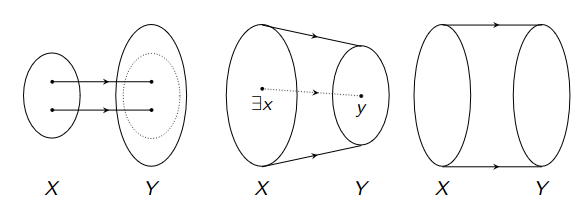
\includegraphics[width=\linewidth]{images/functions.png}
% \end{figure}
\end{dfn}
\vspace{-5pt}

\begin{dfn}[Graph Isomorphisms]{def:graph-iso}{1.1.3}
    An \textbf{isomorphism} between two graphs is a \textit{bijection} between them that preserves all edges. More precisely, if $\Gamma_{1}$ and $\Gamma_{2}$ are graphs, with sets of vertices $V_{1}$ and $V_{2}$ respectively, then an isomorphism from $\Gamma_{1}$ and $\Gamma_{2}$ is a bijection
    \[f : V_{1}\to V_{2}\]
    such that $f(v_{1})$ and $f(v_{2})$ are joined by an edge if and only if $v_{1}$ and $v_{2}$ are also joined by an edge.
    We say that $\Gamma_{1}$ and $\Gamma_{2}$ are \textit{isomorphic} if there exists an isomorphism $f:\Gamma_{1}\to\Gamma_{2}$
\end{dfn}
\vspace{-5pt}

\begin{dfn}[Symmetry]{def:symmetry}{1.1.9}
    A \textbf{symmetry} of a graph is an \textit{isomorphism} from the graph to itself, i.e. if the set of vertices is V, then the symmetry is a bijection $f:V\to V$ that preserves edges. That is, a symmetry is a bijection $f:V\to V$ such that $f(v_{1})$ and $f(v_{2})$ are joined by an edge if and only if $v_{1}$ and $v_{2}$ are joined by an edge.
\end{dfn}
\vspace{-5pt}

% -------------------------------------

\subsection*{Groups}

\begin{dfn}[Groups]{def:group-def}{1.2.3}
    For an operation $\ast$, We say a non-empty set G is a \textbf{group} under $\ast$ if the following four axioms hold:
    \renewcommand\labelitemi{\tiny$\bullet$}
    \begin{itemize}
        \setlength\itemsep{0em}
        \item \textbf{G1 - Closure:} $\ast$ is a binary operation on G, that is $a\ast b \in G$ for all $a,b\in G$.
        \item \textbf{G2 - Associativity:} $(a\ast b) \ast c =a\ast(b\ast c)$ for all $a,b,c\in G$
        \item \textbf{G3 - Identity:} There exists an \textit{identity} element of $G$ such that $e\ast g = g\ast e = g$ for all $g\in G$.
        \item \textbf{G4 - Inverse:} Every element $g\in G$ has an \textit{inverse} $g^{-1}$ such that $g\ast g^{-1}=g^{-1}\ast g = e$
    \end{itemize}
\end{dfn}
\vspace{-5pt}

\begin{dfn}[Abelian Group]{def:abelian}{1.2.6}
    The definition of a group doesn't require that $a\ast b = b\ast a$.
    We say that a group is \textbf{abelian} or \textbf{commutative} if $a\ast b = b\ast a$ for every $a,b\in G$. We say that $a$ \textit{commutes} with $b$, or that $a$ and $b$ \textit{commute}
\end{dfn}
\vspace{-5pt}

% TODO: Examples of groups
% Dihedral, Symmetric, Product Group, Sets of numbers

% -------------------------------------

\subsection*{Subgroups}

\begin{dfn}[Subgroups]{def:subgroup-def}{2.1.1}
    Let $G$ be a group. We say that a non-empty subset $H$ of $G$ is a \textbf{subgroup} of $G$ if $H$ itself is a group (under the operation from $G$). We write $H\le G$ if $H$ is a subgroup of $G$. If $H\ne G$, we write $H<G$ and say $H$ is a proper subgroup
\end{dfn}
\vspace{-5pt}

\begin{thm}[Subgroup Test]{thm:subgroup-test}{2.1.3}
    $H\subseteq G$ is a subgroup of $G$ if and only if:
    \renewcommand\labelitemi{\tiny$\bullet$}
    \begin{itemize}
        \setlength\itemsep{0em}
        \item \textbf{S1:} $H$ is not empty
        \item \textbf{S2:} If $h,k\in H$ then $h\ast k\in H$
        \item \textbf{S3:} If $h\in H$ then $h^{-1}\in H$
    \end{itemize}
    Alternative test for subgroups:
    \renewcommand\labelitemi{\tiny$\bullet$}
    \begin{itemize}
        \setlength\itemsep{0em}
        \item $\widetilde{S1}$: $H$ is not empty.
        \item $\widetilde{S2}$: If $h,k\in H$ then $h*k^{-1}\in H$
    \end{itemize}
\end{thm}
\vspace{-5pt}

\begin{dfn}[Order of an Element]{def:element-order}{2.2.4}
    Let $G$ be a group and $g\in G$. Then the \textbf{order} $o(g)$ of $g$ is the \textit{least} natural number $n$ such that
    $$g^n = e$$
    If no such $n$ exists, we say that $g$ has infinite order
\end{dfn}
\vspace{-5pt}

\begin{dfn}[Order of a Group]{def:group-order}{2.2.3}
    The \textbf{order} of a finite group, written $\lvert G \rvert$, is the number of elements in $G$.
    If $G$ is infinite we say that $\lvert G \rvert = \infty$, or the order of $G$ is infinite.
\end{dfn}
\vspace{-5pt}

\begin{thm}[Order of a Finite Group]{thm:finite-order-thm}{2.2.6}
    In a finite group, every element has finite order.\newline
    If $g$ is an element of a finite group $G$, then there exists $k\in \N$ such that $g^{k} = g^{-1}$
\end{thm}
\vspace{-5pt}

\begin{dfn}[Generating Subset]{def:generator}{2.2.8}
    Let $G$ be a group and let $g\in G$ be an element. We define the subset
    $$\langle g \rangle := \{g^k \mid k\in\mathbb{Z}\} = \{\dots,\,g^{-2},\,g^{-1},\,e,\,g,\,g^{2},\,\dots \}$$
    Note that if $G$ is finite, then by \ref{thm:finite-order-thm} $\langle g \rangle$ is finite, and we can think of $\langle g \rangle$ as
    $$\langle g \rangle = \{e,\,g,\,\dots,\,g^{o(g)-1}\}$$
\end{dfn}
\vspace{-5pt}

\begin{dfn}[Cyclic Subgroup]{def:cyclic-subgroup}{2.2.10}
    A subgroup $H\le G$ is \textbf{cyclic} if $H = \langle h \rangle$ for some $h\in H$. In this case, we say that $H$ is the \textit{cyclic subgroup generated by h}. If $G=\langle g \rangle$ for some $g\in G$, then we say that the group $G$ is \textit{cyclic}, and that $g$ is a \textit{generator}.
\end{dfn}
\vspace{-5pt}

\begin{rem}[Consequences of Cyclic groups]{rem:cyclic-consequences}{2.2.12 - 16}
    \renewcommand\labelitemi{\tiny$\bullet$}
    \begin{itemize}
        \setlength\itemsep{0em}
        \item \textbf{2.2.12} If $g\in G$, then $o(g)=\lvert \langle g \rangle \rvert$
        \item \textbf{2.2.13:} If $G$ is cyclic, then $G$ is abelian.
        \item \textbf{2.2.14:} Let $G$ be a finite group. Then
        \[G \text{ is cyclic } \iff G \text{ has an element of order} \lvert  G\rvert \]
        \item \textbf{2.2.15:} Let $G$ be a cyclic group and let $H$ be a subgroup of $G$. Then $H$ is cyclic.
        \item \textbf{2.2.16:} Let $m,n\in \N$, let $G=\langle g \rangle$ be a cyclic group of order $m$ and $H=\langle h \rangle$ be a cyclic group of order $n$. Then
        $$G \times H \text{ cyclic} \iff m \text{ and } n \text{ are coprime (gcd(m,n) = 1)}$$
    \end{itemize}
\end{rem}
\vspace{-5pt}

% -------------------------------------

\subsection*{Cosets and Lagrange}

\begin{dfn}[Relation]{def:relation}{2.3.2}
    Let $X$ be a set, and $R$ a subset of $X\times X$; thus $R$ consists of some ordered pairs $(s,t)$ with $s,t\in X$. If $(s,t) \in R$ we write $s \sim t$ and say "$s$ is related to $t$". We call $\sim$ a \textbf{relation} on $X$.
\end{dfn}
\vspace{-5pt}

\begin{dfn}[Equivalence Relation]{def:equiv-relation}{2.3.2}
    \renewcommand\labelitemi{\tiny$\bullet$}
    \begin{itemize}
        \setlength\itemsep{0em}
        \item \textbf{Reflexive:} $x\sim x$ for all $x\in X$
        \item \textbf{Symmetric:} $x\sim y$ implies that $y\sim x$ for all $x,y\in X$
        \item \textbf{Transitive:} $x\sim y$ and $y\sim z$ implies that $x\sim z$ for all $x,y,z\in X$
    \end{itemize}
    A relation $\sim$ is called an \textbf{equivalence relation} on X if it satisfies the following three axioms:  
\end{dfn}
\vspace{-5pt}

\begin{dfn}[Coset]{def:coset}{2.3.4}
    Let $H\le G$ and let $g\in G$. Then a \textit{left coset} of  $H$ in $G$ is a subset of $G$ of the form $gH$, for some $g\in G$.
    We denote the set of left cosets of $H$ in $G$ by $G/H$
\end{dfn}
\vspace{-5pt}

\begin{thm}[Lagrange's Theorem]{thm:lagrange}{2.4.2}
    Suppose that $G$ is a finite group.
    \renewcommand\labelitemi{\tiny$\bullet$}
    \begin{itemize}
        \setlength\itemsep{0em}
        \item If $H\le G$, then $\lvert  H\rvert $ divides $\lvert G\rvert $
        \item Let $g\in G$. Then $o(g)$ divides $\lvert  G\rvert $
        \item For all $g\in G$, we have that $g^{\lvert G\rvert } = e$
    \end{itemize}
\end{thm}
\vspace{-5pt}

\newpage

% -------------------------------------
% =====================================
% -------------------------------------

\begin{thm}[Coset Rules]{thm:coset-rules}{2.3.8}
Let $H\le G$
\renewcommand\labelitemi{\tiny$\bullet$}
\begin{itemize}
    \setlength\itemsep{0em}
    \item For all $h\in H$, $hH = H$. In particular $eH = H$
    \item For $g_{1}, g_{2}\in G$, the following are equivalent
    \renewcommand\labelitemi{\tiny$\bullet$}
    \begin{itemize}
        \setlength\itemsep{0em}
        \item $g_{1}H = g_{2}H$
        \item there exists $h\in H$ such that $g_{2} = g_{1}h$
        \item $g_{2}\in g_{1}H$
    \end{itemize}
    \item For $g_{1},\,g_{2}\in G$, define $g_{1}\sim g_{2}$ if and only if $g_{1}H=g_{2}H$. Then $\sim$ defines an equivalence relation on $G$.
\end{itemize}
\end{thm}
\vspace{-5pt}

\begin{thm}[Index of a Subgroup]{thm:subgroup-index}{2.4.4}
The \textbf{index} of $H\le G$ is defined as the number of \textit{distinct} left cosets of $H$ in $G$, which by Lagrange's is $\lvert G / H\rvert = \frac{\lvert G\rvert}{\lvert H\rvert }$
\end{thm}
\vspace{-5pt}

\begin{rem}[Consequences of Lagrange]{rem:lagrange-consequences}{2.4.6 - 8}
\renewcommand\labelitemi{\tiny$\bullet$}
\begin{itemize}
    \setlength\itemsep{0em}
    \item \textbf{2.4.6:} Suppose that $G$ is a group with $\lvert G \rvert=p$, where $p$ is prime. Then $G$ is a cyclic group
    \item \textbf{2.4.7:} Suppose that $G$ is a group with $\lvert G \rvert < 6$. Then $G$ is abelian
    \item \textbf{2.4.8:} If $p$ is a prime and $a\in \Z$, then $a^{p} \equiv a \mod{p}$
\end{itemize}
\end{rem}
\vspace{-5pt}

\subsection*{Homomorphisms and Isomorphisms}
\begin{dfn}[Group Homomorphism]{def:homomorphism}{3.1.1}
    Let $(G,*),(H,\circ)$ be groups. A map $\phi:G\to H$ is called a \textbf{homomorphism} if
    $$\phi(x*y)=\phi(x)\circ\phi(y)\quad \text{for all } x,y\in G$$
    Note that the product on the left is formed using $\ast$, while the product on the right is formed using $\circ$
\end{dfn}
\vspace{-5pt}

\begin{dfn}[Group Isomorphism]{def:group-iso}{3.1.2}
    A group homomorphism $\phi:G\to H$ that is also a bijection is called an \textbf{isomorphism} of groups. In this case we say that $G$ and $H$ are \textit{isomorphic} and we write $G\cong H$. 
    An isomorphism $G\to G$ is called an \textbf{automorphism} of $G$.
\end{dfn}
\vspace{-5pt}

\begin{thm}[Cyclic Isomorphisms]{thm:cyclic-isos}{3.1.L}
All finite cyclic groups of the same order are \textit{isomorphic} to each other. Therefore, cyclic groups of order $n$ are isomorphic to $(\Z_{n}, +)$
\vspace{0pt}\newline
All infinite cyclic groups are \textit{isomorphic} to each other. Therefore, each cyclic group of infinite order is isomorphic to $(\Z, +)$
\end{thm}
\vspace{-5pt}



\begin{rem}[Consequences of Homomorphisms]{rem:homo-consequences}{3.1.5}
Let $\phi:G\to H$ be a group homomorphism. Then
\renewcommand\labelitemi{\tiny$\bullet$}
\begin{itemize}
    \setlength\itemsep{0em}
    \item $\phi(e_{G})=e_{H}$
    \item $\phi(g^k)=(\phi(g))^{k}$ and $\phi(g^{-1})=(\phi(g))^{-1}$ for all $g\in G$
    \item If $\phi$ is injective, the order of $g\in G$ equals the order of $\phi(g)\in H$.
\end{itemize}
\end{rem}
\vspace{-5pt}

\begin{dfn}[Normal Subgroup]{def:normal-subgroup}{3.1.7}
    A subgroup $N\le G$ is \textbf{normal} if the left and right cosets of $N$ are equal, i.e. $gN = Ng$ for all $g\in G$. If $N$ is a normal subgroup of $G$, we write $N\triangleleft G$. Kernels of homomorphisms are always normal subgroups
\end{dfn}
\vspace{-5pt}

\begin{dfn}[Image and Kernel of a Group]{def:img-ker}{3.1.6}
    Let $\phi:G\to H$ be a group homomorphism.
    \renewcommand\labelitemi{\tiny$\bullet$}
    \begin{itemize}
        \setlength\itemsep{0em}
        \item The \textbf{image} of $\phi$ is defined to be
        \[\Ima{\phi} := \{h\in H\,|\,h=\phi(g)\text{ for some } g\in G\}\]
        \item The \textbf{kernel} of $\phi$ is defined to be
        \[\ker{\phi}:= \{g\in G\,|\,\phi(g) = e_{H}\}\]
    \end{itemize}
    Note: $\Ima{\phi}$ is a subgroup of $H$ and $\ker{\phi}$ is a subgroup of $G$
\end{dfn}
\vspace{-5pt}

\begin{thm}[Product Isomorphisms]{thm:prod-isos}{3.2.1}
Let $H,K\le G$ be subgroups with $H\cup K = \{e\}$.
\renewcommand\labelitemi{\tiny$\bullet$}
\begin{itemize}
    \setlength\itemsep{0em}
    \item The map $\phi:H\times K\to HK$ given by $\phi:(h,k)\to hk$ is bijective
    \item If every element of $H$ commutes with every element of $K$ when multiplied in $G$ (i.e. $hk=kh\quad \forall h\in H, k\in K$), then $HK$ is a subgroup of $G$, and it is isomorphic to $H\times K$ via $\phi$
\end{itemize}
\end{thm}
\vspace{-5pt}

\begin{thm}[Size of Product Group]{thm:prodgroup-size}{3.2.3}
Let $H,K\le G$ be finite subgroups of a group $G$ such that $H\cup K = \{e\}$ Then $\lvert HK\rvert =\lvert H\rvert \times \lvert K\rvert $.
\end{thm}
\vspace{-5pt}


\subsection*{Group Actions}

\begin{dfn}[Group Action]{def:action}{4.1.1}
    Let $(G,*)$ be a group, and let $X$ be a nonempty set. Then a (left) \textbf{action} of $G$ on $X$ is a map
    \[G\times X\to X\]
    written $(g,x)\mapsto g\cdot x$, such that
    \[g_{1}\cdot(g_{2}\cdot x) = (g_{1} * g_{2}) \cdot x \qquad \text{and} \qquad e\cdot x = x \]
    for all $g_{1},g_{2}\in G$ and all $x\in X$.
\end{dfn}
\vspace{-5pt}

\begin{dfn}[Kernel of an Action, Faithful Action]{def:action-kernel-faith}{4.1.4}
Suppose that $G$ acts on $X$. Then the set
\[N := \{g\in G\mid g\cdot x=x \forall x\in X\}\]
is a subgroup of $G$, and is called the \textbf{kernel} of the action. If $N = \{e\}$, then we say the action is \textbf{faithful}
\end{dfn}
\vspace{-5pt}

\begin{dfn}[Orbit, Stabilizer, and Fix]{def:orbit}{4.2.1}
    For every $x$ in $X$, the \textbf{orbit} of $x$ is defined by
    \[\text{Orb}_{G}(x)=\{g\cdot x \mid g\in G\}\]
    This is a subset of $X$
    \vspace{0pt}\newline
    For every $x$ in $X$, the \textbf{stabilizer} of $x$ is defined by
    \[\text{Stab}_{G}(x)=\{g\in G : g\cdot x = x\}\]
    This is a subgroup of $G$
    \vspace{0pt}\newline
    For every $g$ in $G$, the \textbf{fix} of $g$ is defined by
    \[\Fix (g) = \{x\in X\mid g\cdot x=x\}\]
    Let $G$ act on $X$, let $x\in X$ and set $H:=\Stab_{G}(x)$. If $y=g\cdot x$ for some $g\in G$, then
    \[\send_{x}(y)=gH\]
\end{dfn}
\vspace{-5pt}

\begin{thm}[Orbit Equivalence]{thm:orbit-equivalence}{4.2.5}
Let $G$ act on $X$. Then
\[x\sim y \iff y = g\cdot x \text{ for some } g\in G\]
defines an equivalence relation on $X$. The equivalence classes are the orbits of $G$. Thus when $G$ acts on $X$, we obtain a partition of $X$ into orbits
\end{thm}
\vspace{-5pt}

\begin{thm}[Orbit-Stabilizer Theorem]{thm:orbit-stab-thm}{4.3.1}
Suppose $G$ is a finite group acting on a set$X$, and let $x\in X$. Then $\lvert \Orb_{G}(x)\rvert \times \lvert \Stab_{G}(x)\rvert = \lvert G\rvert$, or in words:
\[\text{size of orbit } \times \text{ size of stabilizer } = \text{order of group}\]
\end{thm}
\vspace{-5pt}

% TODO: wtf is this?
\begin{thm}[Orbit Send Theorem]{thm:orbit-send}{4.3.4}
Let $G$ act on $X$, let $x \in X$, and let set $H:= \Stab_{G}(x)$. Then the map
$$\send_{x}: \Orb_{G}(x)\to G/H \text{ which sends } y\mapsto \send_{x}(y)$$
\end{thm}
\vspace{-5pt}

\begin{thm}[Cauchy's Theorem]{thm:cauchy}{4.4.2}
Let $G$ be a group, $p$ be prime. If $p$ divides $\lvert G\rvert $, then $G$ contains an element of order $p$
\end{thm}
\vspace{-5pt}
\newpage

% ========================== %
%                            %
%          ANALYSIS          %
%                            %
% ========================== %

\section{\huge Analysis}
\subsection*{Real Numbers and Bounds}
\begin{dfn}[The Real Numbers]{def:reals}{1.1}
$\R$ is defined as the set of real numbers. It has two operations $+$ and $\ast$, and it is a field, i.e. satisfies group axioms for both, in addition the Distributive law:
\[a\cdot(b+c) = a\cdot b + a\cdot c\]
\vspace{0pt}\newline
The set of real numbers is also ordered, i.e. there is a relation $<$ which satisfies pretty much what you think it does
\vspace{0pt}\newline
Finally, the set of real numbers is complete, i.e. there are no gaps between any numbers.
\end{dfn}
\vspace{-5pt}

\begin{dfn}[Suprema and Bounds]{def:suprema}{1.3.2}
Let $E \subset \R$ be nonempty
\vspace{-5pt}
\renewcommand\labelitemi{\tiny$\bullet$}
\begin{itemize}
    \setlength\itemsep{0em}
    \item The set $E$ is said to be bounded above if there is $M\in R$ such that $a\le M$ for all $a\in E$
    \item A real number $M$ is called an upper bound of the set$E$ if $a\le M$ for all $a\in E$
    \item A real number $s$ is called the \textbf{supremum} of the set $E$ if 
    \vspace{-5pt}
    \renewcommand\labelitemi{\tiny$\bullet$}
    \begin{itemize}
        \setlength\itemsep{0em}
        \item $s$ is an upper bound of $E$
        \item $s\le M$ for all upper bounds $M$ of the set $E$
    \end{itemize}
    If a number $s$ exists, we shall say that $E$ has a supremum and write $s=\sup E$
\end{itemize}
If the supremum $s$ exists, then $s$ is the least upper bound of the set $E$. The supremum is also unique if it exists.
\end{dfn}
\vspace{-5pt}

\begin{dfn}[Infimum]{def:infimum}{1.3.10}
If the same properties as a supremum apply but in the other direction, a number $s$ is instead called the \textbf{infimum} of the set $E$. Infimum and Supremum are related via the reflection principle:
\renewcommand\labelitemi{\tiny$\bullet$}
\begin{itemize}
    \setlength\itemsep{0em}
    \item Set $E$ has a supremum if and only if the set $-E$ has an infimum. Also $\inf (-E) = -\sup(E)$
    \item Set $E$ has an infimum if and only if the set $-E$ has a supremum. Also $\sup (-E) = -\inf(E)$
\end{itemize}
\end{dfn}

\begin{thm}[Suprema Approximation Property]{thm:sup-approx-property}{1.3.5}
If the set $E \subset \R$ has a supremum then for any positive number $\epsilon > 0$ there exists $a \in E$ such that
\[\sup E - \epsilon < a \le \sup E\]
\end{thm}
\vspace{-5pt}

%remark 1.3.6 : if e sset N has a supremum then supE in E

\begin{thm}[Archimedean Principle]{thm:archi-principle}{1.3.7}
Given positive real numbers $a,b\in \R$ there is an integer $n \in N$ such that $b<na$
\end{thm}
\vspace{-5pt}

\begin{dfn}[Countability]{def:countability}{1.5.2}
Let $E$ be a set. $E$ is said to be:
\vspace{-5pt}
\renewcommand\labelitemi{\tiny$\bullet$}
\begin{itemize}
    \setlength\itemsep{0em}
    \item \textbf{Finite} if either $E=\varnothing$, or there is an integer $n\in \N$ and a bijection $f : \{1,\, 2,\, 3,\, \dots ,\, n\} \to E$. We say that the set $E$ has $n$ elements
    \item \textbf{Countable} if there is a bijective function $f:\N\to E$
    \item \textbf{At most countable} if $E$ is finite or countable
    \item \textbf{Uncountable} if $E$ is neither finite nor countable
\end{itemize}
Additionally, a nonempty set $E$ is at most countable if and only if there is a surjective function $f:\N\to E$
\end{dfn}
% TODO: this needs some mega cut downs

\subsection*{Sequences and Series}

\begin{dfn}[Convergence of a Sequence]{def:sequence-convergence}{2.1.1}
A sequence of real numbers $(x_{n})$ is said to converge to a real number $a$ if for every $\epsilon>_{0}$ there is a $N\in \N$ where for every $n\ge N$ we have that $\lvert x_{n}- a \rvert < \epsilon $
%TODO diff ways of saying if there is space
\end{dfn}
\vspace{-5pt}

\begin{dfn}[Bounds of Sequences]{def:sequence-bounds}{2.1.9}
Let $(x_{n})$ be a sequence of real numbers.
\vspace{-5pt}
\renewcommand\labelitemi{\tiny$\bullet$}
\begin{itemize}
    \setlength\itemsep{0em}
    \item $(x_{n})_{n\in \N}$ is said to be \textbf{bounded above} if $x_{n} \le M$ for some $M\in\R$ and all $n\in \N$
    \item $(x_{n})_{n\in \N}$ is said to be \textbf{bounded below} if $x_{n} \ge m$ for some $m\in\R$ and all $n\in \N$
    \item $(x_{n})_{n\in N}$ is said to be \textbf{bounded} if it is both bounded above and below
\end{itemize}
\end{dfn}
\vspace{-5pt}

\begin{rem}[Limit Theorems]{rem:limit-thms}{2.2.1 - ?}
\renewcommand\labelitemi{\tiny$\bullet$}
\begin{itemize}
    \setlength\itemsep{0em}
    \item Let $E\subset \R$. If $E$ has a finite supremum then there is a sequence $(x_{n})$ with each $x_{n}\in E$ such that $x_{n}\to \sup E$ as $n\to \infty$. The same goes for a finite infimum
    \item \textbf{Comparison Theorem for sequences:} Suppose that $(x_{n})$, $(y_{n})$ are real sequences. If both $\lim_{n\to \infty} x_{n}$, $\lim_{y\to \infty} y_{n}$ exist and belong to $\R*$, and if $x_{n}\le y_{n}$ for all $n\ge N$ for some $N\in \N$, then $\lim_{n\to \infty} x_{n} \le \lim_{n\to \infty} y_{n}$
\end{itemize}
\end{rem}
\vspace{-5pt}

\begin{dfn}[Monotone Sequences]{def:monotone-seqs}{2.3.1}
    Let $(s_{n})$ be a sequence of real numbers.
    \renewcommand\labelitemi{\tiny$\bullet$}
    \begin{itemize}
        \setlength\itemsep{0em}
        \item $(s_{n})$ is said to be increasing if $s_{1}\le s_{2}\le s_{3}\le\cdots$, and strictly increasing if $s_{1}<s_{2}<s_{3}<\cdots$
        \item $(s_{n})$ is said to be decreasing if $s_{1}\ge s_{2}\ge s_{3}\ge\cdots$, and strictly decreasing if $s_{1}>s_{2}>s_{3}>\cdots$
        \item $(s_{n})$ is said to be monotone if it is either increasing or decreasing
    \end{itemize}
\end{dfn}
\vspace{-5pt}

%TODO: maybe include definition of convergence for limits

\begin{thm}[Top 10 Limit Theorems]{thm:limit-theorems}{lots}
\renewcommand\labelitemi{\tiny$\bullet$}
\begin{itemize}
    \setlength\itemsep{0em}
    
    \item \textbf{Squeeze Theorem (for sequences):} Suppose that $(x_{n})$, $(y_{n})$, and $(w_{n})$ are real sequences
    \vspace{-5pt}
    \renewcommand\labelitemi{\tiny$\bullet$}
    \begin{itemize}
        \setlength\itemsep{0em}
        \item If both $x_{n}\to a$ and $y_{n} \to a$ as $n\to\infty$, and if $x_{n}\le w_{n}\le y_{n}$ for all $n\ge N_{0}$, then $w_{n}\to a$ as $n\to\infty$
        \item If $x_{n}\to 0$ and $(y_{n})$ is bounded, $x_{n}y_{n}\to_{0}$ as $n\to\infty$
    \end{itemize}
    \vspace{-5pt}
    
    \item \textbf{Divergence Test:}
    \vspace{-5pt}
    \renewcommand\labelitemi{\tiny$\bullet$}
    \begin{itemize}
        \setlength\itemsep{0em}
        \item If $\sum^{\infty}_{n=1} a_n$ converges, then $a_n\to0$.
        \item If $(a_n)_{n\in\N}$ doesn't converge to $0$, then $\sum_{n=1}^{\infty} a_n$ diverges. Be careful that the converse isn't true.
    \end{itemize}
    \vspace{-5pt}
    
    % \item \textbf{Bounded Theorem:} Let $(a_{n})_{n\in \N}$ be a sequence with non-negative terms. The following are equivalent:
    % \renewcommand\labelitemi{\tiny$\bullet$}
    % \vspace{-5pt}
    % \begin{itemize}
    %     \setlength\itemsep{0em}
    %     \item The series $\sum_{n=1}^{\infty} a_{n}$ converges
    %     \item The sequence $(s_{n})_{n\in \N}$ of partial sums is bounded above
    % \end{itemize}
    % \vspace{-1pt}
    
    \item \textbf{Comparison Test:} Let $(a_n)_{n\in\N}$ and $(b_n)_{n\in\N}$ be two sequences such that $0\leq a_n\leq b_n$ for all n.
    \renewcommand\labelitemi{\tiny$\bullet$}
    \vspace{-5pt}
    \begin{itemize}
        \setlength\itemsep{0em}
        \item If $\sum_n b_n$ converges, then $\sum_n a_n$ converges as well.
        \item If $\sum_n a_n$ diverges, then $\sum_n b_n$ diverges as well.
    \end{itemize}
    \vspace{-5pt}

    \item \textbf{Limit Comparison Test:} Let $(a_n)_{n\in\N}$ and $(b_n)_{n\in\N}$ be two real sequences with $a_n\geq0$ and $b_n > 0$ for all n. Assume that $a_n / b_n \to L$ for some $L\in(0,\infty)$. Then, $\sum_{n=1}^{\infty}  a_n$ converges iff $\sum_{n=1}^{\infty}  b_n$ converges. 
    \renewcommand\labelitemi{\tiny$\bullet$}
    \vspace{-5pt}
    \begin{itemize}
        \setlength\itemsep{0em}
        \item If $L=0$ and $\sum_{n=1}^{\infty}b_{n}$ converges then $\sum_{n=1}^{\infty} a_{n}$ converges
        \item If $L=\infty$ and $\sum_{n=1}^{\infty}a_{n}$ diverges then $\sum_{n=1}^{\infty} b_{n}$ diverges
    \end{itemize}
    \vspace{-5pt}
    
    \item \textbf{Root Test:} Let $\sum_{n=0}^{\infty} a_n$ be a series with non-negative terms such that $\sqrt[n]{a_n} \to L$ where $0 \le L \le +\infty$.
    \renewcommand\labelitemi{\tiny$\bullet$}
    \vspace{-5pt}
    \begin{itemize}
        \setlength\itemsep{0em}
        \item If $0\le L < 1$ then the series $\sum_{n=0}^{\infty}  a_n$ converges.
        \item If $L > 1$ then the series $\sum_{n=0}^{\infty}  a_n$ diverges.
        \item If $L = 1$, the series may or may not converge
    \end{itemize}
    \vspace{-5pt}

    \item \textbf{Ratio Test:} Let $\sum_{n=0}^{\infty}  a_n$ be a series with positive terms such that $(a_{n+1}) / (a_n) \to L$, where $0\le L \le +\infty$.
    \renewcommand\labelitemi{\tiny$\bullet$}
    \vspace{-5pt}
    \begin{itemize}
        \setlength\itemsep{0em}
        \item If $0\le L < 1$ then the series $\sum_{n=0}^{\infty}  a_n$ converges.
        \item If $L > 1$ then the series $\sum_{n=0}^{\infty}  a_n$ diverges.
        \item If $L = 1$ then compare to $p$ series
    \end{itemize}
    \vspace{-5pt}

    \item \textbf{Cauchy's Condensation Test:} Let $(a_n)_{n\in\N}$ be a decreasing sequence with non-negative terms. Then the following are equivalent:
    \vspace{-5pt}
    \renewcommand\labelitemi{\tiny$\bullet$}
    \begin{itemize}
        \setlength\itemsep{0em}
        \item The series $\sum_{n=1}^{\infty}  a_n$ converges
        \item The series $\sum_{n=0}^{\infty}  2^na_{2^n}$ converges.
    \end{itemize}
    \vspace{-5pt}

    \item \textbf{Alternating Series Test:} Let $(b_n)_{n\in\N}$ be a \textit{decreasing} sequence of non-negative real numbers that converges to zero. Then the series $\sum_{n=1}^{\infty} (-1)^{n-1}b_n$ converges.
    
    \item \textbf{Monotone Convergence Theorem:} If a sequence of real numbers $(s_{n})$ is increasing and bounded above, or decreasing and bounded below, then $(s_{n})$ is convergent (and converges to the supremum/infinum of the set $\{x_{n}\,\vert\,n\in\N\}$ respectively).
    
    \item \textbf{Geometric Series Test:} Assume $a,\,r\in\R, a,\,r\ne 0$. Then
    \[\displaystyle\sum_{n=1}^{\infty} a\cdot r^n = \begin{cases}
    \dfrac{a}{1-r} &\text{if } \lvert r \rvert < 1 \\
    \text{diverges} &\text{if } \lvert r \rvert \ge 1
    \end{cases}
    \]
    Notice that $a$ is always the first term in the series, and $r$ is the \textit{common ratio}
    \vspace{-1pt}
\end{itemize}
\end{thm}
\vspace{-5pt}

\newpage

\subsection*{Continuity and Functional Limits}

\begin{dfn}[Continuity]{def:continuity-def}{4.1.1}
    Let $f$ be a real-valued function whose domain is a subset of $\R$. The function $f$ is \textbf{continuous} at $x_{0}$ in $\dom{(f)}$ if, for every sequence $(x_{n})$ in $\dom{(f)}$ converging to $x_{0}$, we have 
    \[\displaystyle\lim_{ n \to \infty }f(x_{n})=f(a)\]
    If $f$ is continuous at each $a\in S \subseteq \dom{(f)}$ and then we say that $f$ is continuous on $S$. If $f$ is continuous on $\dom{(f)}$ then we say that $f$ is continuous
\end{dfn}
\vspace{-5pt}

\begin{thm}[$\epsilon-\delta$ Definition of Continuity]{thm:e-d-continuity}{4.1.6}
    A function $f:A\to\R$ is continuous if for all $\epsilon>0$, there exists some $\delta>0$ s.t. for all $x \in A$ for which $0<\lvert x-c \rvert <\delta$, we have 
    \[\lvert f(x)-f(c) \rvert < \epsilon\]
\end{thm}
\vspace{-5pt}

\begin{thm}[Evil $\epsilon-\delta$ definition of continuity]{thm:negated-e-d-continuty}{6.1.4}
    A function $f:A\to\R$ is not continuous if there exists $\epsilon>0$ such that for all $\delta>0$ there exists some $x \in A$ satisfying $0<\lvert x-c \rvert<\delta$ for which $\lvert  f(x)-f(c) \rvert\ge \epsilon$
\end{thm}
\vspace{-5pt}

\begin{dfn}[Bounds of a Function]{def:function-bounds}{4.2.1}
Let $E\subseteq\R$ be nonempty. A function $f:E\to \R$ is said to be bounded on $E$ if
\[\lvert f(x)\rvert \le M,\qquad \text{for all } x\in E\]
where $M$ is some (large) real number.
\end{dfn}
\vspace{-5pt}

% TODO: what is the point of this :D
\begin{thm}[Extreme Value Theorem]{thm:ext-val-thm}{4.2.2}
Let $I\subseteq \R$ be a closed and bounded interval. Let $f:I\to \R$ be continuous on $I$. Then $f$ is bounded on the interval $I$, denoted by
\[m = \inf\{f(x)\mid x\in I\},\qquad M = \sup\{f(x)\mid x\in I\}\]
Then there exist points $x_{m}, x_{M}\in I$ such that
\[f(x_{m}) = m \quad \text{and} \quad f(x_{M}) = M\]
\end{thm}
\vspace{-5pt}

\begin{thm}[$\epsilon-\delta$ Limit jr.]{thm:mini-e-d-limit}{4.2.4}
Let $f: I\to \R$ where $I$ is an open nonempty interval. If $f$ is continuous at a point $a\in I$ and $f(a)> 0$ then for some $\delta,\,\epsilon> 0$ we have that
\[f(x)>\epsilon,\quad \text{ for all } x\in (a-\delta, a+\delta)\]
\end{thm}
\vspace{-5pt}

\begin{thm}[Intermediate Value Theorem]{thm:intermediate-value}{4.2.5}
Let $I$ be a non-degenerate interval and let $f:I\to\R$ be a continuous function. If $a,b\in I,\,a<b$, then on the interval $(a,b)$, $f$ attains all values between $f(a)$ and $f(b)$. i.e. given $y_{0}$ between $f(a)$ and $f(b)$, there exists $x_{0}\in(a,b)$ such that $f(x_{0}) = y_{0}$
\end{thm}
\vspace{-5pt}

\begin{thm}[Bolzano's Theorem]{thm:bolzano}{4.2.6}
Let $f(x)$ be continuous on $[a,b]$ such that $f(a)f(b) < 0$, then there exists $c\in (a,b)$ such that $f(c)$ = 0
\end{thm}
\vspace{-5pt}

\begin{thm}[$\epsilon-\delta$ definition of a limit]{thm:e-d-limit}{4.3.1}
    Let $f:A\to\R$ and let $c$ be a limit point of $A$. Then we say that
    \[\displaystyle\lim_{x \to c} f(x) = L\]
    if for all $\epsilon>0$ there exists some $\delta>0$ such that for every $x\in A$ for which $0<\lvert x-c \rvert<\delta$, we have
    \[\lvert f(x)-L \rvert<\epsilon \]
    We also say $\displaystyle\lim_{x \to c}f(x)$ \textbf{converges} to L in such a situation
\end{thm}
\vspace{-5pt}

% TODO: some more interval theorems that could be added

\subsection*{Differentiation}
\begin{dfn}[First Principle Differentiation]{def:first-principles}{5.1.1}
A real function $f$ is said to be differentiable at a point $a\in \R$ if $f$ is defined at some open interval containing $a$, and
\[f'(a) = \lim_{x\to a} \frac{f(x) - f(a)}{x - a}\]
exists. $f'(a)$ is called the derivative of $f$ at the point $a$
\end{dfn}
\vspace{-5pt}

% \begin{dfn}[Tangent to a graph]{def:tangent-diff}{5.1.?}
%     If $f$ is differentiable at $x_{0}$ then the straight line given by
%     \[y=f(x_{0}) + f'(x_{0})(x-x_{0})\]
%     is called the tangent to the graph of $f$ at $(x_{0},f(x_{0}))$.
% \end{dfn}
% \vspace{-5pt}

\begin{thm}[Differentiable implies Continuous]{thm:diff-to-conti}{5.1.3}
    Let $I$ be an open interval, $x_{0}\in I$ and $f:I\to \R$ be differentiable at $x_{0}$. Then $f$ is continuous at $x_{0}$. The converse is not true, an example is $f(x)=\lvert x\rvert $ which isn't differentiable at $0$.
\end{thm}
\vspace{-5pt}

\begin{thm}[Differentiable Intervals]{thm:diff-intervals}{5.1.4}
    Let $f:I\to \R$ be a given fucntion, where $I$ is an open interval. We say that $f$ is differentiable in $I$ iff it is differentiable at every point in $I$.
    At endpoints, derivatives only have to be one-sided
\end{thm}
\vspace{-5pt}

\begin{thm}[Differentiation Rules]{thm:diff-rules}{5.2.1}
    Let $f,g:(a,b)\to \R$ be differentiable on $(a,b)$. Then $f+g$ and $f\cdot g$ are differentiable on $(a,b)$. If $g(x)\ne 0$ for all $x \in (a,b)$, then $f/g$ is differentiable. Moreover,
    \vspace{-5pt}
    \renewcommand\labelitemi{\tiny$\bullet$}
    \begin{itemize}
        \setlength\itemsep{0em}
        \item \textbf{Sum rule:} $(f+g)' = f' + g'$
        \item \textbf{Product Rule:} $(fg)'=f'g + fg'$
        \item \textbf{Quotient Rule:} $\left(f / g\right)' =(f'g - fg') /g^{2}$
    \end{itemize}
\end{thm}
\vspace{-5pt}

\begin{thm}[Inverse Function Theorem]{thm:invs-func}{5.4.6}
    Let $f$ be injective and continuous on an open interval $I$. If $a\in f(I)$ and $f'$ at the point $f^{-1}(a)\ne 0$ exists and is nonzero, then $f^{-1}$ is differentiable at $a$ and
    \[(f^{-1})'(a)= \frac{1}{f'(f^{-1}(a))}\]
\end{thm}
\vspace{-5pt}


% \subsection*{The progressively more generalised Theorem ladder}

\begin{thm}[Chain Rule]{thm:chain-rule}{5.2.2}
    Let $f,\,g$ be real functions. If $f$ is differentiable at $a$ and $g$ is differentiable at $f(a)$ then $g\circ f$ is differentiable at $a$ and
    \[(g\circ f)'(a) = g'(f(a))f'(a)\]
\end{thm}
\vspace{-8pt}

\begin{thm}[Differentiation Theorem ladder]{thm:rolles}{5.3.1 - 3}
    \renewcommand\labelitemi{\tiny$\bullet$}
    \begin{itemize}
        \setlength\itemsep{0em}
        \item \textbf{Rolle's Theorem:} Let $a,b\in \R,\,a<b$. If $f:[a,b] \to \R$ is continuous in $[a,b]$, differentiable in $(a,b)$ and $f(a)=f(b)$, then there exists a point $c$ in $(a,b)$ such that $f'(c)=0$
        \item \textbf{Mean Value Theorem:} If $f:[a,b]\to\R$, $a<b$ is continuous in $[a,b]$, differentiable in $(a,b)$ then $\exists c\in (a,b)$ s.t.
        \[f'(c)=\frac{f(b)-f(a)}{b-a}\]
        \item \textbf{Generalised MVT:} If $f,g:[a,b]\to\R$ is continuous in $[a,b]$ and differentiable in $(a,b)$, then $\exists c$ in $(a,b)$ such that
        \[(f(b)-f(a))g'(c)=(g(b)-g(a))f'(c)\]
        If $g(b)-g(a),\,g'(c)\ne 0$ then this can be written as
        \[\frac{f(b)-f(a)}{g(b)-g(a)}= \frac{f'(c)}{g'(c)}\]
    \end{itemize}
\end{thm}
\vspace{-8pt}

\begin{thm}[Monotone Functions]{thm:monotone-functions}{5.4.2}
Let $a<b$ be real and $f$ be continuous on $[a,b]$ and differentiable on $(a,b)$.
\renewcommand\labelitemi{\tiny$\bullet$}
\begin{itemize}
    \setlength\itemsep{0em}
    \item If $f'(x) > 0\,\, \forall x\in (a,b)$, then $f$ is strictly increasing on $[a,b]$
    \item If $f'(x) < 0\,\, \forall x\in (a,b)$, then $f$ is strictly decreasing on $[a,b]$
    \item If $f'(x) = 0\,\, \forall x\in(a,b)$, then $f$ is constant on $[a,b]$
\end{itemize}
Additionally, if $f$ is injective and continuous on an interval $I$, Then $f$ and $f^{-1}$ is strictly monotone on $I$ and $f(I)$ respectively
\end{thm}
\vspace{-8pt}

\begin{thm}[Taylor Series]{thm:taylor-remainder}{5.5.1}
    Let $f:I\to\R$ be $n+1$ times differentiable and $x_{0}\in I$, for an open interval $I$. For each $x \in I$, there is a $c$ between $x_{0}$ and $x$ such that
    \[f(x)=\sum_{k=0}^{n} \frac{f^{(k)}(x_{0})}{k!} (x-x_{0})^k + \frac{f^{(n+1)}(c)}{(n+1)!}(x-x_{0})^{n+1}\]
    (c depends on $x$ and $n$)
    \vspace{0pt}\newline
    Now suppose that $f:(a,b)\to\R$ is infinitely differentiable and let $x_{0}\in (a,b)$. Fix $x$ in $(a,b)$. For every positive integer $N$ we have
    \[f(x)=\sum_{k=0}^{N} \frac{f^{(k)}(x_{0})}{k!}(x-x_{0})^{k} + R_{N}(x)\]
    If $R_{N}(x) \to 0$ as $n\to\infty$, we have
    \[f(x) = \sum_{k=0}^{\infty} \frac{f^{(k)}(x_{0})}{k!}(x-x_{0})^{k}\]
\end{thm}
\vspace{-8pt}
Made by Leon
\newpage

\section{Examples Catalogue}

\subsection*{Geometric Examples of a Group}

\begin{xmp}[Dihedral Group $D_{n}$]{ex:dihedral}{1.2.4}
The set of symmetries of an $n$-gon forms a group under composition. We call this group the \textbf{Dihedral Group} $D_{n}$
\vspace{0pt}\newline
The Dihedral group of $n$ has precisely $\lvert D_{n} \rvert = 2n$ elements, namely
\renewcommand\labelitemi{\tiny$\bullet$}
\begin{itemize}
    \setlength\itemsep{0em}
    \item The identity $e$
    \item $n- 1$ anticlockwise rotations of $\frac{2pi}{n}$. We denote this operation with $g$
    \item $n$ reflections. If $n$ is odd, then there are $n$ reflections from a point to the opposite edge. If $n$ is even, there are $\frac{n}{2}$ reflections from point to point, and $\frac{n}{2}$ from edge to edge. We denote a vertical reflection with $h$, and rotated reflections as compositions of $h$ and $g$ 
\end{itemize}
From this, we see that
\[D_{n} = \{e,\,g,\,g^{2},\,\dots,\,g^{n-1},\, h,\, gh,\, g^{2}h,\,\,\dots,\, g^{n-1}h \}\]
\end{xmp}
\vspace{-5pt}

\begin{xmp}[Symmetric Group]{ex:symmetric-group}{1.3.2}
The set of all symmetries of $\{1,\, 2,\,\dots,\,n\}$ is called the \textbf{symmetric group} $S_{n}$. It is a group under composition with order $\lvert S_{n}  \rvert = n!$ The symmetric group can be thought of as every permutation of the set $\{1,\, 2,\,\dots,\,n\}$, or can also be thought of as an $n$-gon where every edge is connected to each other. 
\end{xmp}
\vspace{-5pt}

% examples of abelian group
% cyclic group

[0,1) 
{a in Q | 0 < a < sqrt2}


\begin{xmp}[Example of a Coset]{ex:coset-example}{?}
    Consider $\Z_{4}$ under addition, and let $H=\{0,2\}$ ($e=0$.) The cosets of $H$ in $G$ are:
    \[\begin{aligned}
    eH = e * H = \{e * h\,|\,h\in H\} = \{0+h\,|\, h\in H\} = \{0,2\} \\
    1H = 1 * H = \{1 * h\,|\,h\in H\} = \{1+h\,|\, h\in H\} = \{1,3\} \\
    2H = 2 * H = \{2 * h\,|\,h\in H\} = \{2+h\,|\, h\in H\} = \{0,2\} \\
    3H = 3 * H = \{3 * h\,|\,h\in H\} = \{3+h\,|\, h\in H\} = \{1,3\}
    \end{aligned}\]

    Hence there are two cosets, namely
    \[0 * H=2 * H=\{0,2\} \quad\text{and}\quad 1 * H=3 * H=\{1,3\}\]
    The above shows that $g_{1}H=g_{2}H$ is possible, even when $g_{1}\ne g_{2}$
    We also have
    \[G/H=\{eH=2H,1H=3H\} = \{\{0,2\}, \{1,3\}\}\]
\end{xmp}
\vspace{-5pt}

\begin{xmp}[p-series]{ex:p-series}{3.3.5}
The series $\displaystyle\sum_{n=1}^{\infty} \frac{1}{k^{p}}$ converges if $p > 1$, and it diverges if $p \le 1$. At $p = 1$, this series is called the \textbf{Harmonic Series}.
\vspace{0pt}\newline
To show divergence/convergence of a series, we can compare it to the p-series

\end{xmp}
\vspace{-5pt}


\begin{xmp}[$\epsilon$-N Convergence]{ex:e-n-convergence}{10000}
    \textit{Show that the sequence $\left( \frac{2n+1}{3n+2} \right)_{n\in\mathbb{N}}$ converges to $\frac{2}{3}$}
    \vspace{0pt}\newline
    We start with the rough work. Start with an arbitrary $\epsilon>0$ and find an $N_{\epsilon}$ s.t. $\left\lvert  \frac{2n+1}{3n+2} -\frac{2}{3}  \right\rvert < \epsilon$ for all $n>N_{\epsilon}$. Let's explore this.
    \[\left\lvert  \frac{2n+1}{3n+2}-\frac{2}{3}  \right\rvert =\frac{11}{3(3n+2)} < \epsilon\quad\implies \quad n> \frac{1}{3}\left( \frac{11}{3\epsilon} -2\right)\]
    \textbf{Proof:} Let $\epsilon>0$. Pick a positive integer $N$ such that
    \[N>\frac{1}{3}\left( \frac{11}{3\epsilon}-2 \right)\]
    Then,
    \[\frac{11}{3(3N+2)} < \epsilon\]
    For all $n$ with $n\ge N$ we have 
    \[\lvert a_{n}-L \rvert = \left\lvert  \frac{2n+5}{3n+2} - \frac{2}{3}  \right\rvert =\frac{11}{3(3n+2)} \le \frac{11}{3(3N+2)}<\epsilon\]
    another method of finding a limit is,
    $$\left\lvert  \frac{2n+1}{3n+2}-\frac{2}{3}  \right\rvert =\frac{11}{3(3n+2)} = \frac{11}{9n+6} < \frac{11}{9n}< \epsilon$$
    Since $9n+6>9n$, this means that the right fraction is larger than the left fraction in all cases. This means if we can find a right fraction that is smaller than $\epsilon$ then the left fraction must also.
    \vspace{0pt}\newline 
    \textbf{Proof:} let $\epsilon>0$. Pick a positive integer $N$ such that $N>\frac{11}{9\epsilon}$. Then $\frac{11}{9N} < \epsilon$. For all $n$ with $n\ge N$, we have
    $$\lvert a_{n}-L \rvert = \left\lvert  \frac{2n+5}{3n+2} - \frac{2}{3}  \right\rvert =\frac{11}{9n+6} \le \frac{11}{9n} \le \frac{11}{9N}<\epsilon$$
\end{xmp}
\vspace{-5pt}

% \begin{xmp}[$\epsilon-\delta$ Continuity]{ex:e-d-continuity}{a}
% \textit{Using the expansion $(x-y)^{3} = (x-y)(x^{2}+ax+a^{2})$, show that the function $f(x) = x^{3}$ is continuous}
% \vspace{0pt}\newline
% Using the definition of continuity, we wcnt to find a $\delta$ such that for all $\epsilon> 0$, all $x\in\R$ where $0 < \lvert x-c\rvert  < \delta$ results in $\lvert f(x) - f(a)\rvert < \epsilon$
% \vspace{0pt}\newline
% Rough work: stcrt off with $\lvert f(x)-f(a)\rvert$
% \[\begin{aligned}
%     \lvert f(x) - f(c)\rvert &< \epsilon\\
%     \lvert x^{3} - c^{3} \rvert &< \epsilon\\
%     \lvert x-c\rvert \lvert x^{2}+ax+a^{2}\rvert &< \epsilon 
% \end{aligned}\]
% If we let $\delta < 1$, then using the triangle inequality,
% \[\lvert x - c\rvert < 1 \quad \implies \lvert x\rvert < 1 + \lvert a\rvert \]
% Now we ccn substitute this back into the equation:
% \[\begin{aligned}
%     \lvert x-c\rvert \lvert x^{2}+ax+a^{2}\rvert &< \lvert x-a\rvert \left( \lvert x \rvert^{2} + \lvert c\rvert \lvert x\rvert +\lvert c\rvert^{2} \right)\\
%     &<\lvert x-c\rvert (\lvert 1 + \lvert a\rvert \rvert^{2} + \lvert c\rvert \lvert 1 + c\rvert + c^{2} ) < \epsilon
% \end{aligned}\]
% Therefore, $\lvert x-c\rvert < \displaystyle \frac{\epsilon}{\lvert 1 + \lvert a\rvert \rvert^{2} + \lvert c\rvert \lvert 1 + c\rvert + c^{2}} = \delta$?
% idk
% \end{xmp}
% \vspace{-5pt}

\begin{xmp}[$\epsilon-\delta$ Continuity]{ex:e-d-continuity}{?}
\textit{Using the definition of continuity, prove that the function $f: \R\backslash \{\frac{9}{5}\}\to \R$ defined by $f(x)=\frac{x^{2}}{5x-9}$ is continuous at $x_{0}= 2$}
Since $x_{0} = 2$, our delta should end up as $\lvert x-2\rvert < \delta$. Start with $\lvert f(x) - f(a)\rvert  < \epsilon$
\[\begin{aligned}
    \lvert f(x)-f(a) \rvert  & = \left\lvert  \frac{x^{2}}{5x-9}-\frac{4}{10-9}  \right\rvert \\
    &=\left\lvert  \frac{x^{2}}{5x-9}-4  \right\rvert \\
    &=\left\lvert  \frac{x^{2}-20x+36}{5x-9}  \right\rvert \\
    &=\left\lvert \frac{(x-18)(x-2)}{5x-9}  \right\rvert  \\
    &= \lvert x-2 \rvert \left\lvert  \frac{x-18}{5x-9}  \right\rvert \\
\end{aligned}\]
We have $\lvert x-2\rvert$, so we want to turn the RH fraction into a constant. If we let the neighbourhood around $\delta$ to be no less than $\frac{1}{10}$ (i.e. $x\in(1.9, 2.1)$) (this number can be anything, but smaller than $\frac{1}{5}$ since there is an asymptote at $\frac{9}{5}$), using the number with the largest value in that range we can get an upper bound for $\delta$.
\[\left\lvert \frac{x-18}{5x-9}\right\rvert < \left\lvert \frac{1.9 - 18}{9.5 - 9}\right\rvert = \left\lvert \frac{-16.1}{0.5} \right\rvert = \left\lvert -32.2 \right\rvert \implies \left\lvert \frac{x-18}{5x-9}\right\rvert < 32.2\]
Therefore
\[\lvert x-2 \rvert \left\lvert  \frac{x-18}{5x-9}  \right\rvert < \lvert x-2 \rvert \cdot 32.2 < \epsilon\]
Therefore, we can take $\delta = \max \{1/10, \epsilon / 32.2\}$
\vspace{0pt}\newline
\textbf{Proof:} Let $\epsilon > 0$ be given. set $\delta = \min\{\frac{1}{10}, \frac{\epsilon}{32.2}\}$. Then for all $x\in \R$ such that $\lvert x - 2\rvert < \delta$ we have
\[\left\lvert \frac{x-18}{5x-9}\right\rvert < \left\lvert \frac{1.9 - 18}{9.5 - 9}\right\rvert = \left\lvert \frac{-16.1}{0.5} \right\rvert = \left\lvert -32.2 \right\rvert \implies \left\lvert \frac{x-18}{5x-9}\right\rvert < 32.2\]
Therefore, since $\left\lvert \frac{x-18}{5x-9}\right\rvert < 32.2$,
\[
    \lvert f(x) - f(a)\rvert = \left\lvert  \frac{x^{2}}{5x-9}-\frac{4}{10-9}  \right\rvert = \left\lvert  \frac{x^{2}-20x+36}{5x-9}  \right\rvert
\]\[
    = \left\lvert \frac{(x-18)(x-2)}{5x-9}  \right\rvert = \lvert x-2 \rvert \left\lvert  \frac{x-18}{5x-9}  \right\rvert \le 32.2 \cdot \lvert x - 2\rvert < 32.2 \cdot \delta = \epsilon
\]

\end{xmp}
\vspace{-5pt}

\begin{xmp}[$\epsilon-\delta$ Continuity Template]{ex:e-d-c-template}{a}
    \textbf{Proof:} Let $\epsilon > 0$ be given. Set $\delta = \text{\underline{\quad}}$. Then for all $x\in \R$ such that $\lvert x - \text{\underline{\quad}}\rvert < \delta$ we have
    \vspace{0pt}\newline
    \textit{Optional: preliminary step to determine an upper bound}
    \vspace{0pt}\newline
    Therefore, / Therefore since $\text{``\underline{x term}''} < \text{``\underline{constant}''}$,
    \vspace{0pt}\newline
    ``Same steps as rough working''
    \[\text{\underline{\quad}} \cdot \lvert x - \text{\underline{\quad}}\rvert < \text{\underline{\quad}}\delta = \epsilon\]
    \end{xmp}
    \vspace{-5pt}

\begin{xmp}[$\epsilon-\delta$ Discontinuity]{ex:discontinuity}{)}
    From negation of $\epsilon-\delta$ continuity - A function $f:A\to\R$ is not continuous if there exists $\epsilon>0$ such that for all $\delta>0$ there exists some $x \in A$ satisfying $0<\lvert x-c \rvert<\delta$ for which $\lvert  f(x)-f(c) \rvert\ge \epsilon$
    \[\lvert f(x) - f(a)\rvert < \epsilon \implies \left\lvert sin\left(\frac{1}{x}\right) - 0 \right\rvert < \epsilon \quad \implies \left\lvert sin\left(\frac{1}{x}\right)\right\rvert < \epsilon\]
    So we want to show that we can find an $\epsilon$ such that for every $\delta > 0$, we can find an $x$ where $\lvert x\rvert < \delta$ and also $\lvert sin(\frac{1}{x})\rvert \ge \epsilon$.
    \vspace{0pt}\newline
    Since $sin(x)$ repeats, if we can find an $x$ such that $sin(\frac{1}{x})$ is an exact value then we can define $\epsilon$ as something lower than that. If we want a value where $sin(\frac{1}{x}) = 1$, this will be true if $x = 1 / (\frac{\pi}{2} + 2N\pi)$, where $N$ is a positive integer.
    \vspace{0pt}\newline
    Since $x$ has to be bounded by $\delta$, go from $\delta$
    \[\begin{aligned}
        \lvert x\rvert  &< \delta\\
        \left\lvert \frac{1}{\frac{\pi}{2}+2N\pi}\right\rvert &< \delta\\
        \frac{1}{\frac{\pi}{2}+2N\pi} &< \delta \quad \text{(will always be positive since N positive int)}\\ 
        \frac{\pi}{2}+2N\pi &> \frac{1}{\delta}\\
        N &> \frac{1}{2\pi}\left( \frac{1}{\delta} - \frac{\pi}{2} \right)
        % \lvert x\rvert  < \delta\quad\implies \left\lvert \frac{1}{\frac{\pi}{2}+2N\pi}\right\rvert < \delta \quad\implies \frac{1}{\frac{\pi}{2}+2N\pi} < \delta\\
        % \implies\frac{\pi}{2}+2N\pi > \frac{1}{\delta} \quad\implies
        % N > \frac{1}{2\pi}\left( \frac{1}{\delta} - \frac{\pi}{2} \right)
    \end{aligned}\]
    \textbf{Proof:} Let $\epsilon = \frac{1}{2}$. Let $\delta > 0$ be given. Pick a positive integer $N$ such that $N > \frac{1}{2\pi}\left( \frac{1}{\delta} - \frac{\pi}{2} \right)$ and set $x = \frac{1}{\frac{\pi}{2} + 2N\pi}$. Then for all $x\in \R$ such that $0 < x < \delta$, we have
    \[\lvert f(x)\rvert = \left\lvert sin\left(\frac{1}{x}\right) \right\rvert = \left\lvert sin\left(\frac{\pi}{2} + 2N\pi\right) \right\rvert = 1 \ge \frac{1}{2} = \epsilon\]
\end{xmp}
\vspace{-5pt}

% absolute convergence

\lipsum[1-12]

\end{multicols}

\end{document}